% !TEX root = prace.tex
\chapter{Teorie dialogových systémů}
\label{ch:kap1}

\section{Dialogový systém}

Dialogový systém je počítačový systém, který umožňuje uživatelům komunikovat s počítačem ve formě, která je přirozená a efektivní pro použití.
Vývoj dialogových systémů má před sebou ještě spoustu problémů k překonání a pro praktické použití je třeba se uchýlit k několika předpokladům a zjednodušením.
Prvním zjednodušením je doménová specializace, v současné době není možné vytvořit dialogový systém, který by se dokázal s uživatelem bavit o libovolném tématu.
Z toho plyne i nutnost ontologie, systém potřebuje databázi popisující všechny informace, které může poskytnout a jejich strukturu.
Systém má definované fráze a věty, které může použít, na rozdíl od živého operátora, který dokáže improvizovat.

Další zjednodušení se týkají přímo dialogu.
Předpokládá se, že dialog probíhá vždy mezi systémem a jedním uživatelem.
Navíc se pravidelně střídají v obrátkách.
Jedna obrátka dialogu je složená z jedné promluvy systému a jedné promluvy uživatele.

Příkladem dialogového systému může být systém pro nalezení spojení pomocí městské dopravy.
Příkaz od uživatele může vypadat např. takto: \uv{Chci jet z Malostranského náměstí na Anděl}.
Dialogový systém z této věty odvodí, že uživatel hledá spojení, výchozí stanice je Malostranské náměstí a cílová stanice je Anděl.
Nyní záleží na chování dialogového systému, může například předpokládat, že uživatel chce vždy najít nejdřívější spojení, pokud neřekne jinak.
V takovém případě už systém může rovnou najít v databázi nejbližší spojení a uživateli jej sdělit.

Důležitou vlastností dialogového systému je robustnost.
Pokud budeme používat dialogový systém v přirozeném prostředí, musíme se vyrovnat s tím, že často nebude uživateli rozumět.
Systém může informaci přeslechnout, anebo si nemusí být jistý tím, co slyšel.
Dialogový systém se proto musí umět uživatele doptat na chybějící informace a musí umět pracovat s nejistotou.

\section{Součásti dialogového systému}

Dialogový systém se skládá z několika částí, které spolu komunikují.
Na vstupu je zvukový záznam uživatele, o jeho převedení do textu se stará systém rozpoznávání řeči (ASR).
Z textu je potřeba získat sémantické informace pomocí systému porozumění mluvené řeči (SLU).
Nad sémanticky anotovanými informacemi už může pracovat dialogový manager (DM), který zvolí patřičnou odpověď.
Výstupem dialogového manageru jsou informace, které se mají předat uživateli.
O jejich převedení do textu se stará systém generování přirozené řeči (NLG).
Do zvukového záznamu převede text syntetizér řeči (TTS).

\subsection{Systém rozpoznávání řeči (ASR)}

Systém rozpoznávání řeči slouží k převedení mluveného projevu do textové podoby.
Až po získání textové podoby je možné se zabývat významem textu.
Aktuálně nejlepší systémy jsou založené na pravděpodobnostním modelu a využívají Skryté Markovské modely (HMM) k určení nejpravděpodobnější sekvence slov pro daný zvukový záznam \cite{juang1991hidden}.
Pro tuto část dialogového systému existuje řada dostupných otevřených toolkitů, např. systém HTK \cite{young2002htk}, Kaldi \cite{Povey_ASRU2011} nebo SPHINX~\cite{walker2004sphinx}.
Existuje i celá řada komerčního software od firem jako IBM nebo Nuance.

Úspěšnost systému rozpoznávání řeči je závislá na obtížnosti úlohy a na počtu trénovacích dat, pocházejících ze stejné domény.
Pro obecnou doménu se problém stává mnohem těžší a je třeba velké množství dat.
Pro měření výkonu ASR systému se používá metrika Word Error Rate (WER).
Pro spočítání WER je třeba nejprve provést zarovnání rozpoznaného a originálního textu.
WER je pak počet slov, která jsou změněná, smazaná, anebo přidaná, vydělený počtem slov v originálním textu.Dialogový systém Let's Go!~\cite{raux2006doing} například dosahuje průměrné WER $64.3\%$.

Systém rozpoznávání řeči může produkovat více hypotéz pro jeden vstup.
Často existuje pro jeden zvukový záznam více možných slovních sekvencí, z kterých by mohl pocházet.
Reprezentace možných hypotéz může být seznam slovních sekvencí s jejich věrohodností.
Věrohodnosti jsou skóre přiřazené hypotézám, které určují jakou důvěru má systém rozpoznávání řeči ve správnost dané slovní sekvence.
Příklad možného seznamu hypotéz je v tabulce~\ref{tab:sezhyp}.

\begin{table}[h]
\begin{center}
\begin{tabular}{|c|l|}
\hline
Věrohodnost & Hypotéza \\
\hline
\hline
0.676 & poliklinika modřany\\
\hline
0.072 & poliklinika\\
\hline
0.063 & cheb poliklinika modřany\\
\hline
0.054 & poliklinika bory\\
\hline
0.045 & poliklinika modřany i\\
\hline
0.036 & polikliniky\\
\hline
0.027 & cheb poliklinika\\
\hline
0.018 & cheb poliklinika bory\\
\hline
0.009 & poliklinika i\\
\hline
\end{tabular}
\end{center}
\caption{Příklad seznamu hypotéz ze systému pro rozpoznávání přirozené řeči.
Uživatel by rád jel do zastávky Poliklinika Modřany.}
\label{tab:sezhyp}
\end{table}

Pro práci s hypotézami je vhodné, aby věrohodnost odpovídala aposteriorní pravděpodobnosti sekvence slov, dáno vstupní zvuk.

Další možností jak reprezentovat výstup je použití konfůzní sítě \cite{bertoldi2005new}.
Konfůzní síť je vážený orientovaný graf, obsahující startovní a konečný vrchol a hrany označené slovy.
Každá cesta ze startovního do konečného vrcholu vede přes všechny ostatní vrcholy.
Váhy hran jsou pravděpodobnosti slova přiřazeného dané hraně.
Hrany mohou obsahovat i prázdné slovo $\epsilon$.
Pravděpodobnost sekvence slov je součinem vah po cestě ze startovního do konečného uzlu.
Výhodou konfůzní sítě je, že umožňuje v komprimované podobě uložit mnohem více hypotéz.
Příklad konfůzní sítě je na obrázku~\ref{fig:konnet}.

\begin{figure}
\begin{center}
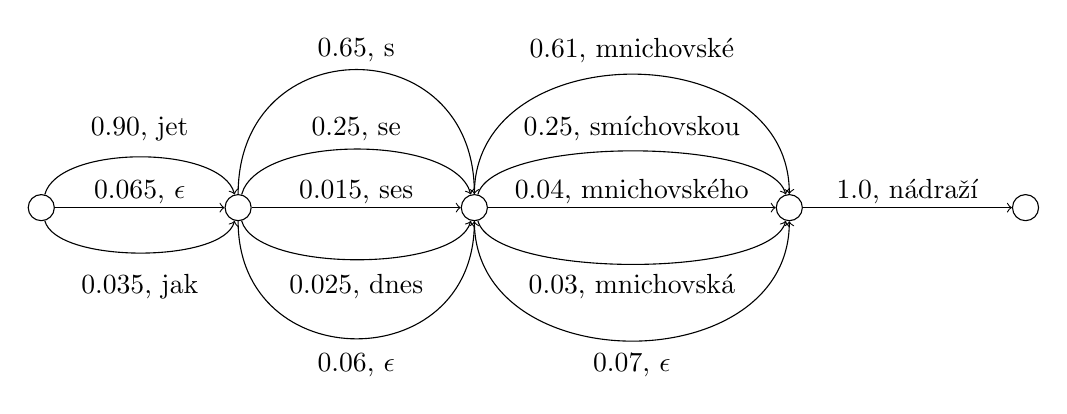
\begin{tikzpicture}[->, main/.style={circle, draw}]


\node[main] at (0,0) (n0) {};
\node[main] at (2.5,0) (n1) {};
\node[main] at (5.5,0) (n2) {};
\node[main] at (9.5,0) (n3) {};
\node[main] at (12.5,0) (n4) {};


\node at (1.25, 1) (a0) {0.90, jet};
\node at (1.25, 0.2) (a1) {0.065, $\epsilon$};
\node at (1.25, -1) (a2) {0.035, jak};

\path[looseness=0.7, out=75, in=105] (n0) edge (n1);
\path (n0) edge (n1);
\path[looseness=0.6, bend right, out=285, in=255] (n0) edge (n1);

\node at (4, 2) (b0) {0.65, s};
\node at (4, 1) (b1) {0.25, se};
\node at (4, 0.2) (b2) {0.015, ses};
\node at (4, -1) (b3) {0.025, dnes};
\node at (4, -2) (b4) {0.06, $\epsilon$};

\path[looseness=1.8, out=90, in=90] (n1) edge (n2);
\path[looseness=0.7, out=75, in=105] (n1) edge (n2);
\path (n1) edge (n2);
\path[looseness=0.6, bend right, out=285, in=255] (n1) edge (n2);
\path[looseness=1.7, bend right, out=270, in=270] (n1) edge (n2);

\node at (7.5, 2) (c0) {0.61, mnichovské};
\node at (7.5, 1) (c1) {0.25, smíchovskou};
\node at (7.5, 0.2) (c2) {0.04, mnichovského};
\node at (7.5, -1) (c3) {0.03, mnichovská};
\node at (7.5, -2) (c4) {0.07, $\epsilon$};

\path[looseness=1.3, out=90, in=90] (n2) edge (n3);
\path[looseness=0.5, out=75, in=105] (n2) edge (n3);
\path (n2) edge (n3);
\path[looseness=0.5, bend right, out=285, in=255] (n2) edge (n3);
\path[looseness=1.3, bend right, out=270, in=270] (n2) edge (n3);

\node at (11, 0.2) (d0) {1.0, nádraží};
\path (n3) edge (n4);

\end{tikzpicture}
\caption{Příklad konfůzní sítě.}
\label{fig:konnet}
\end{center}
\end{figure}

\subsection{Porozumění mluvené řeči (SLU)}

Po získání hypotéz o promluvě uživatele se musi dialogový systém pokusit porozumět, co se uživatel snažil sdělit.
Dialogový systém nepotřebuje vědět, co přesně uživatel řekl, důležité je pouze zjistit význam sdělení.
Pokud například uživatel řekne "Chtěl bych nalézt spojení z Malostranského náměstí na Anděl", anebo "Jak se dostanu na Anděl ze zastávky Malostranské náměstí?", tak pro dialogový systém jsou obě tvrzení ekvivalentní, uživatel požaduje informace o spojení mezi dvěma zastávkami, i když v jednom případě jde o větu oznamovací a v druhém případě o otázku.

První rozdělení mezi přesným významem sdělení a jeho účelem se objevilo ve formě tzv. speech aktů~\cite{austin1975things}.
Následně byla idea speech aktů rozšířena pro potřeby dialogových systémů~\cite{traum1999speech} a výsledek byl nazván dialogovým aktem.

V této práci používáme definici dialogového aktu, která byla použita v soutěži Dialog State Tracking Challenge~\cite{williamsdialog}.
Semántická reprezentace sdělení uživatele se tedy nazývá dialogový akt (DA), skládá se z jedné nebo více položek dialogového aktu (DAI), které jsou spojené v konjunkci.
Každá DAI se skládá z typu, názvu slotu a jeho hodnoty. Typy jsou doménově nezávislé, sloty a jejich hodnoty reprezentují koncepty ontologie.
Příklad dialogového aktu ze systému pro hledání spojení v městské dopravě:

\begin{center}
{\tt hello(), inform(route="61a")}.
\end{center}

Zde se dialogový akt skládá ze dvou položek, první položka má pouze typ {\em hello}, značící pozdrav.
Druhá položka má typ {\em inform}, tzn. uživatel nás informuje o svém požadavku.
Název slotu je {\em route} a hodnota je \uv{61a}, tedy uživatel nám říká, že hledá spojení linkou 61a.

Typů může být libovolné množství, ale existuje několik základních, jejichž použití je ustálené.
\begin{itemize}
\item {\em inform} --- sdělujeme informaci, doplňujeme hodnotu do slotu,
\item {\em request} --- požadujeme od protějšku doplnění hodnoty pro dotazovaný slot,
\item {\em confirm} --- chceme potvrdit hodnotu slotu, potvrzení může být implicitní, anebo explicitní.
	Při explicitním potvrzení očekáváme odpověď \uv{Ano} nebo \uv{Ne},
	U implicitního, pokud se nám nedostane odpovědi předpokládáme, že protějšek souhlasí.
\end{itemize}

V tabulce~\ref{tab:dstcdat} jsou ukázány všechny typy dialogových aktů, které může uživatel říct v dialogovém systému Let's Go!~\cite{williamsdialog}.

\begin{table}
\begin{center}
\begin{tabular}{|l|}
\hline
Typ dialogového aktu \\
\hline
\hline
hello \\
\hline
bye \\
\hline
goback \\
\hline
restart \\
\hline
null \\
\hline
repeat \\
\hline
nextbus \\
\hline
prevbus \\
\hline
tellchoices \\
\hline
affirm \\
\hline
negate \\
\hline
deny \\
\hline
inform \\
\hline
\end{tabular}
\caption{Typy dialogových aktů, které může říct použít uživatel v systému Let's Go!}
\label{tab:dstcdat}
\end{center}
\end{table}

Existuje široké množství technik, které lze použít pro porozumění mluvené řeči.
Unifikace pomocí šablon anebo gramatiky jsou příklady ručně psaných metod.
Metody založené na datech jsou například Hidden Vector State model~\cite{he2005semantic}, techniky strojového překladu~\cite{wong2007learning}, Combinatory Categorical Grammars~\cite{zettlemoyer2007online} nebo Support Vector Machines~\cite{mairesse2009spoken}.

\subsection{Dialogový manager (DM)}

Pokud už jsou pravděpodobné dialogové akty dekódovány, je třeba rozhodnout, jak bude systém reagovat.
Komponenta tvořící rozhodnutí o dalším kroku systému se nazývá dialogový manager.
Odpověď systému je zakódována do formy dialogových aktů a nazývá se systémová akce.

Zvolená systémová akce je vybrána z množiny možných akci $a \in \mathcal{A}$ a závisí na vstupu, který systém obdržel z SLU.
Tento vstup se nazývá pozorování $o \in \mathcal{O}$, protože obsahuje vše, co systém pozoroval o uživateli.

Zvolení správné akce potřebuje více znalostí než jen poslední pozorování.
Celá historie dialogu a také kontext hrají důležitou roli.
Dialogový manager bere na vše ohled pomocí udržovaní interní reprezentace celého pozorovaného dialogu.
Tato reprezentace se nazývá dialogový stav, nebo také stav důvěry, značí se $b \in \mathcal{B}$.
Aktuální dialogový stav závisí na přechodové funkci, která dialogový stav aktualizuje pro každé nové pozorování a systémovou akci.
Přechodová funkce je tedy mapování $\mathcal{T} : \mathcal{B} \times \mathcal{A} \times \mathcal{O} \longrightarrow \mathcal{B}$.
V této práci se budeme věnovat právě metodám aktualizace dialogového stavu.

Chování dialogového stavu definuje dialogová strategie $\pi$.
Strategie určuje co má systém provést v závislosti na aktuálním dialogovém stavu.
Obecně strategie vytvoří pravděpodobnostní rozložení přes možné akce.
Pokud $\prod(\mathcal{A})$ značí množinu těchto distribucí, pak dialogová strategie bude zobrazení z dialogového stavu do této množiny, $\pi: \mathcal{B} \longrightarrow \prod(\mathcal{A})$.

Pozorování, dialogový stav a akce jsou číslovány podle obrátky.
Pokud je časový okamžik důležitý, jsou pozorování, dialogový stav a akce z obrátky číslo $t$ označeny $o_t$, $b_t$ a $a_t$.

\subsection{Generování přirozené řeči (NLG a TTS)}

Posledním krokem dialogového systému je vytvoření odpovědi pro uživatele.
Nejprve systém generování přirozené řeči (NLG) převede dialogové akty na text.
Následně je text převeden na zvuk pomocí textového syntetizéru řeči (TTS).

Nejjednodušším přístup ke generování přirozeného jazyka z dialogových aktů je použití šablon.
Například pro dialogový akt {\tt inform(from.stop="x")} bude vytvořena šablona \uv{Pojedete ze zastávky x}, kde \uv{x} bude nahrazeno například za \uv{Malostranská}, \uv{Letňany}, atd.
Šablony jsou jednoduché a často efektivní řešení, protože počet možných frází je většinou dostatešně malý.

Při syntéze řeči existuje mnoho alternativ.
Je možné použít segmenty řeči z databáze pro vygenerování zvuků tvořících dohromady celou sekvenci slov.
Příkladem těchto systémů je Festival~\cite{black2001festival} nebo jeho odnož  FLite~\cite{black2001flite}.

Alternativní metodou syntézy je použití Skrytých Markovských modelů pro generování zvuku, příkladem je HTS systém~\cite{zen2007hmm}.

Pro syntézu řeči existují také komerční systémy, například systém SpeechTech TTS~\cite{speechtech}.

\section{Dialogový stav}

Dialogový stav je reprezentace všech informací, které lze o aktuálním dialogu získat.
To znamená všechno co uživatel a systém řekl.
Ovšem nejistota v tom, co vlastně uživatel řekl a jaké jsou jeho cíle, je základním problémem, s kterým se dialogový systém musí vypořádat.
Systémy pro rozpoznávání i porozumění řeči často chybují a tuto možnost musí brát dialogový manager také v potaz.
Vypořádat se s nejistotou lze pomocí jejího zakomponování do modelu pro odhad dialogového stavu.

Cíle uživatele a další vlastnosti prostředí lze považovat za náhodné částečně pozorovatelné proměnné a je možné je odvodit z pozorování.
Pravděpodobnostní rozložení těchto náhodných proměnných dává dobře definovanou reprezentaci nejistoty, navíc je možné je reprezentovat pomocí Bayesovské sítě.

Jedním z možných modelů dialogového stavu je generativní model.
Definujeme množinu dialogových stavů, $s \in \mathcal{S}$.
Předpokládáme, že pozorování závisí podmíněně pouze na stavu prostředí a definujeme pravděpodobnostní rozdělení pro pozorování, $p(o \mid s)$.
Dále předpokládáme, že cíle uživatele se nemění v čase a stav prostředí je tedy závislý pouze na stavu v předchozí obrátce a na poslední akci systému.
Tato závislost je zachycena v přechodové pravděpodobnosti $p(s_{t+1} \mid s_t, a_t)$.
Předpoklad, že dialogový stav závisí pouze na minulé hodnotě se nazývá Markovská vlastnost.

Pokud vezmeme předchozí předpoklady, tak lze využít bayesovský přístup pro počítání s nejistotou.
Stav v čase $t$ označíme $s_t$.
Podle Bayesova vzorce můžeme spočítat pravděpodobnost stavu v čase $t+1$ po přijetí nového pozorování $o_{t+1} = o^\prime$.

\begin{equation}
p(s_{t+1} = s^\prime) \propto
    \sum_{s \in \mathcal{S}}
        p(s_t = s)
        p(s_{t+1} = s^\prime \mid s_t = s, a_t = a) p(o_{t+1} = o^\prime \mid s_{t+1} = s^\prime)
\label{eq:beliefupdate}
\end{equation}

Nyní můžeme definovat stav důvěry v čase $t$, $b_t$, jako pravděpodobnost přes stavy dáno všechna pozorování až do času $t$.
Množina všech možných stavů důvěry je pravděpodobnost přes všechny možné dialogové stavy $\mathcal{B} = \prod(\mathcal{S})$.

Můžeme přepsat rovnici~\eqref{eq:beliefupdate} s pomocí stavů důvěry.

\begin{equation}
b(s_{t+1}) \propto
    \sum_{s \in \mathcal{S}}
        b(s_t)
        p(s_{t+1} \mid s_t, a_t)
        p(o_{t+1} \mid s_{t+1})
\label{eq:beliefupdate2}
\end{equation}

Rovnice~\eqref{eq:beliefupdate2} nám dává předpis pro přechodovou funkci $\mathcal{T}$.
V praxi ovšem bude množina možných hodnot pro stav $s_t$ příliš velká, protože stav musí obsahovat všechny informace potřebné pro rozhodování, to znamená celou historii dialogu a cíle uživatele. 
Pokud systém obsahuje sloty, tak každá kombinace hodnot slotu je jedním možným cílem uživatele. 
Tedy velikost stavového prostoru roste exponenciálně.

\subsection{Aktualizace stavu}

Efektivní metodou pro aktualizaci dialogového stavu je použití dynamických bayesovských sítí~\cite{thomson2008bayesian}.
Bayesovské sítě umoňují efektivní výpočet využitím podmíněných nezávislostí mezi sloty.
Stále ovšem zůstává problém s výpočtem, pokud i jednotlivé sloty obsahují příliš mnoho hodnot.
Lze použít aproximace a počítat jen s $k$ nejpravděpodobnějšími hodnotami~\cite{thomson2010bayesian}.

Alternativním zjednodušením je rozdělit stav prostředí do skupin. 
Tento přístup se nazývá Hidden Information State (HIS)~\cite{young2010hidden}.
Základním předpokladem zde musí být, že uživatel nezmění svůj cíl v průběhu dialogu.
Pak lze efektivně provádět aktualizaci, protože rovnice pro aktualizace pravděpodobnosti se nemění mezi jednotlivými skupinami.

V této práci se budeme zabývat prvním přístupem, tedy použitím Bayesovských sítích.
Pro inferenci použijeme Loopy Belief Propagation (LBP) algoritmus, který je aproximativní metodou pro sítě s diskrétními náhodnými proměnnými.
Pro učení parametrů představíme Expectation Propagation (EP) algoritmus.
EP je zobecněním LBP na libovolné pravděpodobnostní rozložení.
